\chapter{Konzeption}
% TODO: weiter schreiben
Dieses Kapitel beinhaltet alle Schritte für die Konzeption der angewandte Methoden. Außerdem wird der Datensatz und die verwendete Frameworks 
präsentiert.

\section{Image Colorization als Multimodales Problem}
Konventionelle automatische Methoden zielen darauf ab, die Farben für ein generiertes Bild so nah wie möglich an das Originale Bild vorherzusagen.
Diese Methoden verwenden ein MSE Loss der Vorhersagen die Weit von den Originalen Farbwerte entfernt liegen, stärker bestraft, als Farbwerte
die dichter an den Originalen Farbwerte liegen. Das führt, wie bei \label{subsection:verwandte-arbeiten} beschrieben, zu entsättigte Bilder.
Die Gründe für diese Ergebnisse ist dass verschiedene Objekte, verschiedene Farben einnehmen können. Aus diesem Grund, behandelt die vorliegende
Arbeit das Problem als ein Multimodales Problem.

\section{Farbraum}
Der Standard Farbraum der Bilder für die Methoden dieser Arbeit ist der RGB-Farbraum. Bei diesem Farbraum lässt sich schwer das Graustufen Bild 
von den Farbkanäle zu trennen, daher wird der Lab-Farbraum verwendet.
\\
\\
Bei den Lab-Farbraum können ohne Probleme die Farbkanäle ``ab'' von den Belichtungskanal ``L'' getrennt werden. Der Belichtungskanal ``L'' 
enthält das Graustufenbild die in den CNN eingespeist wird. Das generierte Bild wird für die Darstellung von dem Lab-Farbraum in den RGB-Farbraum 
konvertiert.

\section{Binning}
Binning ist eine Technik, die für die Bildverarbeitung verwendet wird. Binning wird, in dem Kontext von Image Colorization, als Eingruppierung 
von naheliegenden Farben definiert. Die Farben werden in gleich große Intervalle aufgeteilt. Diese Intervalle bezeichnet man im Englischen als
``\gls{bin}s''. Jedes dieser Intervalle wird durch einen \gls{bin} Index repräsentiert, somit reduziert sich die Anzahl der Klassen die vorhergesagt werden
können.

Als Beispiel für die Veranschaulichung wird der normalisierte Lab-Farbraum in 36 gleich große \gls{bin}s unterteilt. Da die Farbinformationen 
in den ``ab'' Farbkanäle kodiert sind, werden nur diese 2 Farbkanäle in \gls{bin}s klassifiziert. Auf dem Bild \ref{image:bins} ist der Farbkanal 
``a'' auf der x-Achse und der ``b'' Farbkanal auf der y-Achse abgebildet. Die Vierecke repräsentieren die \gls{bin}s. Die obere Zahl in den Bins 
symbolisiert den Index auf dem \gls{grid}, die untere Zahl symbolisiert den Bin Index. Der Index auf den \gls{grid} ist Bedeutsam für die Berechnung der Bins.

\begin{figure}[H]
  \centering
  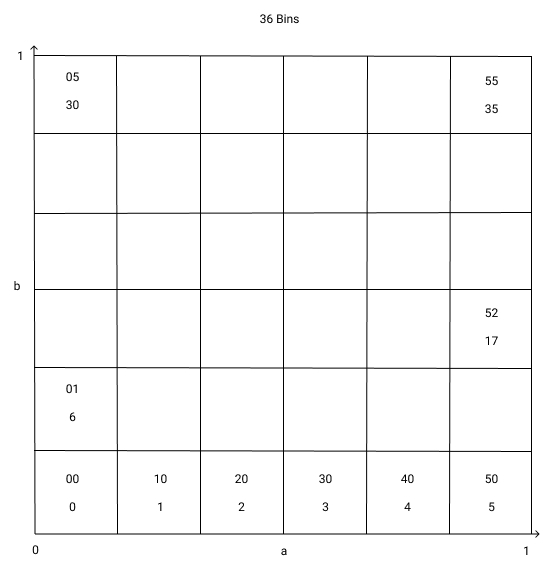
\includegraphics[width=0.55\textwidth]{resources/bins/bins.jpg}
  \caption{
    \gls{grid} mit 36 bins. Die x-Achse bildet die Werte von dem Farbkanal ``a'' und die y-Achse die Werte von den Farbkanal ``b'' ab.
  }
  \label{image:bins}
\end{figure}

Für die Methoden dieser Arbeit wurden nur symmetrische \gls{grid}s verwendet, so ergibt zum Beispiel ein $6 \times 6$ Grid 36 Bins und 
ein $18 \times 18$ Grid 324 Bins.

\section{Netzwerkarchitektur}
TODO
\section{Datensätze}
TODO
\section{Framework}